% Apr 29 2020 - Simple example of a mechanical system with springs drawn with TikZ
\documentclass[10pt,a4paper]{article}
\usepackage[margin=2.5cm]{geometry}
\usepackage[utf8]{inputenc}

\usepackage{tikz}
\usetikzlibrary{decorations}  % Needed for spring zigzags
\usetikzlibrary{decorations.pathmorphing}  % Needed for spring zigzags

\author{Onur Serin}
\title{Some Spring Figures}

% Definitions:
\tikzstyle{spring}=[thick,decorate,decoration={zigzag,pre length=0.1cm,post length=0.1cm,segment length=6}]
\tikzstyle{spring_compressed}=[thick,decorate,decoration={zigzag,pre length=0.1cm,post length=0.1cm,segment length=4}]
\tikzstyle{spring_stretched}=[thick,decorate,decoration={zigzag,pre length=0.1cm,post length=0.1cm,segment length=8}]
%%%

\begin{document}

\begin{center}
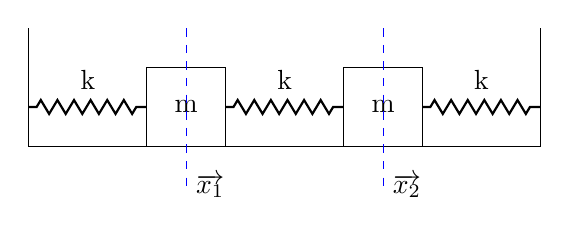
\begin{tikzpicture}

\draw[spring] (0,-1) -- (1.5,-1);
\draw[spring] (2.5,-1) -- (4,-1);
\draw[spring] (5,-1) -- (6.5,-1);
\draw (0.75, -0.65) node {k};
\draw (3.25, -0.65) node {k};
\draw (5.75, -0.65) node {k};

\draw (0,0)
      to  (0,-1.5)
      to  (6.5,-1.5)
      to  (6.5,0);

\draw (1.5,-1.5) rectangle (2.5,-0.5) node[pos=0.5] {m};
\draw [blue,dashed] (2,0)
      to  (2,-2) node[right,black] {$\overrightarrow{x_1}$};

\draw (4.0,-1.5) rectangle (5,-0.5) node[pos=0.5] {m};
\draw [blue,dashed] (4.5,0)
      to  (4.5,-2) node[right,black] {$\overrightarrow{x_2}$};
\end{tikzpicture}
Lorem ipsum\\
\end{center}

\begin{center}
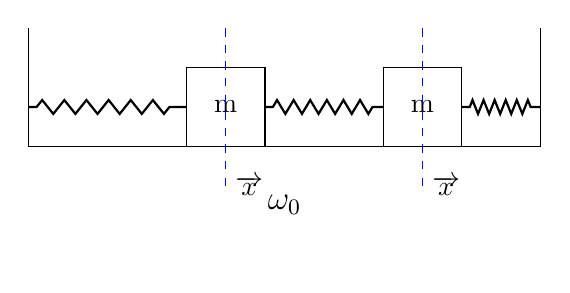
\begin{tikzpicture}  % x_1 = x_2 case

\draw[spring_stretched] (0,-1) -- (2,-1);
\draw[spring] (3,-1) -- (4.5,-1);
\draw[spring_compressed] (5.5,-1) -- (6.5,-1);

\draw (0,0)
      to  (0,-1.5)
      to  (6.5,-1.5)
      to  (6.5,0);

\draw (2,-1.5) rectangle (3,-0.5) node[pos=0.5] {m};
\draw [blue,dashed] (2.5,0)
      to  (2.5,-2) node[right,black] {$\overrightarrow{x}$};

\draw (4.5,-1.5) rectangle (5.5,-0.5) node[pos=0.5] {m};
\draw [blue,dashed] (5,0)
      to  (5,-2) node[right,black] {$\overrightarrow{x}$};

\draw [white] (3.25,-1.75)
      to  (3.25,-2) node[below,black] {\large{$\omega_0$}};

\draw [white] (3.25,-2.5) to (3.25,-3);  % Just some padding
\end{tikzpicture}\\

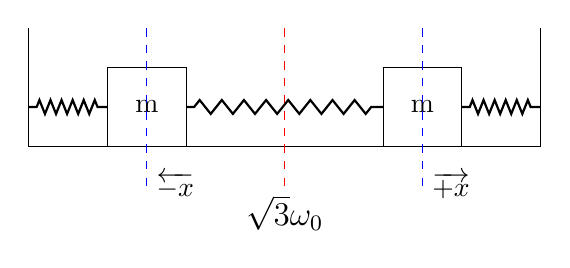
\begin{tikzpicture}  % x_1 = -x_2 case

\draw[spring_compressed] (0,-1) -- (1,-1);
\draw[spring_stretched] (2,-1) -- (4.5,-1);
\draw[spring_compressed] (5.5,-1) -- (6.5,-1);

\draw (0,0)
      to  (0,-1.5)
      to  (6.5,-1.5)
      to  (6.5,0);

\draw (1,-1.5) rectangle (2,-0.5) node[pos=0.5] {m};
\draw [blue,dashed] (1.5,0)
      to  (1.5,-2) node[right,black] {$\overleftarrow{-x}$};

\draw (4.5,-1.5) rectangle (5.5,-0.5) node[pos=0.5] {m};
\draw [blue,dashed] (5,0)
      to  (5,-2) node[right,black] {$\overrightarrow{+x}$};

\draw [red,dashed] (3.25,0)
      to  (3.25,-2) node[below,black] {\large{$\sqrt{3}\omega_0$}};
\end{tikzpicture}
\end{center}

\end{document}
